%%%%%%%%%%%%%%%%%%%%%%%%%%%%%%%%%%%%%%%%%%%%%%%%%%%%%%%%%%%%%%%%%%%%%%%%%%%%%%%%
%2345678901234567890123456789012345678901234567890123456789012345678901234567890
%        1         2         3         4         5         6         7         8

%\documentclass[letterpaper, 10 pt, conference]{ieeeconf}  % Comment this line out
                                                          % if you need a4paper
\documentclass[a4paper, 10pt, conference]{ieeeconf}      % Use this line for a4
                                                          % paper

\IEEEoverridecommandlockouts                              % This command is only
                                                          % needed if you want to
                                                          % use the \thanks command
\usepackage{epsf,graphicx}
\usepackage{latexsym,amssymb}
\usepackage{setspace,cite}
\usepackage{etoolbox}
\usepackage{graphicx}
\usepackage{amsmath,amssymb} % define this before the line numbering.
\usepackage{color}

\overrideIEEEmargins
% See the \addtolength command later in the file to balance the column lengths
% on the last page of the document

\title{\LARGE \bf
Object Flow
}

\author{
Juan Manuel Perez Rua, Tomas Crivelli and Patrick Perez% <-this % stops a space
\thanks{This was supported by Technicolor R\&D}
\thanks{ \noindent {\tt\small juanmanuel.perezrua@technicolor.com}, {\tt\small tomas.crivelli@technicolor.com}, {\tt\small patrick.perez@technicolor.com} }
}
\begin{document}



\maketitle
\thispagestyle{empty}
\pagestyle{empty}


%===========================================================

\begin{abstract}

Superpixels and over segmentation techniques
became a widely used pre-processing stage for a
large number of machine vision applications, after the
original concept was introduced \cite{c1}. Superpixels are
traditionally used as performance booster for several
other techniques. However, it is still mostly related to
single frame processing \cite{c1}\cite{c10}\cite{c11}. In the search for
consistency in superpixel labeling through video,
some authors have proposed different techniques,
which go from simple extension to supervoxels\cite{c9}\cite{c11},
to more complicated approaches \cite{c8}. These
approaches, nonetheless, usually require a global
processing and knowledge of all (or several of) the
video frames beforehand. In this paper we propose a superpixel
matching technique which assumes a flowlike
behavior in the image sequences (natural video), and
propose an application for improving object segmentation in videos.

\end{abstract}
\section{Introduction}
\label{sec:introduction}

Object tracking and optical flow are two of the main components in the
computer vision toolbox, and have been focus of great research efforts, 
leading to significant progress in the last years \cite{c16,c17}. 
The object tracking problem in videos consists on estimating the 
position of a target in every frame, given an initial position. On the
other hand, the optical flow between a pair of frames consists on finding a displacement vector 
for each pixel of the first image, namely a {\it dense motion  or displacement field}. Even though for several
applications a complete (i.e. for every pixel) motion-field is needed, other applications like
human-computer interaction, object editing in video or structure-from-motion,
may only focus on an interest object and thus, only a subset of motion vectors is required. 
In such scenarios combining optical flow and object tracking in a unified 
framework appears useful and the precision of the object motion description 
could be enhanced. For instance, even with modern optical flow approaches, 
the long term dense motion estimation remains a challenge \cite{c20,c22}.  At large, object trackers provide a more robust, 
longer term motion estimation featuring a global description of an object, specially after recent works based on tracking-by-detection approaches \cite{c16,c23,c24}. 
On the other side, they lack the (sub) pixel precision of dense optical flow estimators, as well as a deeper use of contextual information for bundle motion 
vector estimation. 
Even more,  object trackers and optical flow give precious hints for other fundamental tools such as 
object segmentation in video. Nevertheless,
these two techniques were not deeply studied in the literature as a unified problem. Though optical flow has been widely used as a motion 
feature for object tracking \cite{c25}, feeding a dense motion estimator with tracking information is not being fully exploited.
This being said, we introduce  a new problem which we call object flow. Thus, for a given object of interest, 
the object flow is the set of displacement vectors for every pixel that belong to the target in a first frame, 
towards another frame of the sequence. In other words, a dense displacement  field constrained to the spatial support of the object. 
Note that by definition this induces a segmentation of the target and of the motion field.

We can define more precisely the object flow by starting with an image sequence, say $I_t, t:0..N-1$, and an initial 
position of the interest object in the first frame of this sequence. Let $\mathcal{R} \in \Omega$ be the region corresponding to the support of the object in the
bi-dimensional grid $\Omega$. Then, the object flow, $\mathcal{O}(x)$,  is defined as $\mathcal{O}(x) = d_{0,t}(x), \forall x \in \mathcal{R}$.

A straightforward solution to this problem would be to compute the optical flow field between a pair of frames, and to apply 
a segmentation mask to recover the desired motion vectors. Nevertheless, this approach carries several 
problems. For example, a globally computed optical flow method can affect small objects motion, because of 
the common use of heavy regularization prior. Moreover, finding the pixels that belong to the interest object in several frames is a difficult problem. 
We propose an approach to reduce these problems.

%The present paper is organized as follows. We describe our pipeline for object flow, including the novel concept of superpixel flow
%in Sec. \ref{sec:desc} and its use in object segmentation in videos. In following
%sections some results showing how 
%the object flow overpass state of the art optical flow methods for object motion flows 
%estimation are discussed. Finally, some insights and conclusions are given.


\section{Algorithm description}
\label{sec:desc}

The Fig. \ref{figurelabel_sys} shows a simplified block diagram of the proposed system. Two details are important, 
the use of the tracker window to initialize a segmentation procedure, and the use of this segmentation over the tracked window 
to perform a more precise motion flow computation in the interest pixels. The dotted line represents the possible interaction 
between precise flow information with the next tracker state. For instance, the current object flow can work as direction hint, and 
the segmentation information can be used to improve the sampling process of the learning stage in several trackers by detection methods \cite{c22}, and 
thus the tracker and motion flow algorithm can work for mutual enhancement.

   \begin{figure}[thpb]
      \centering
      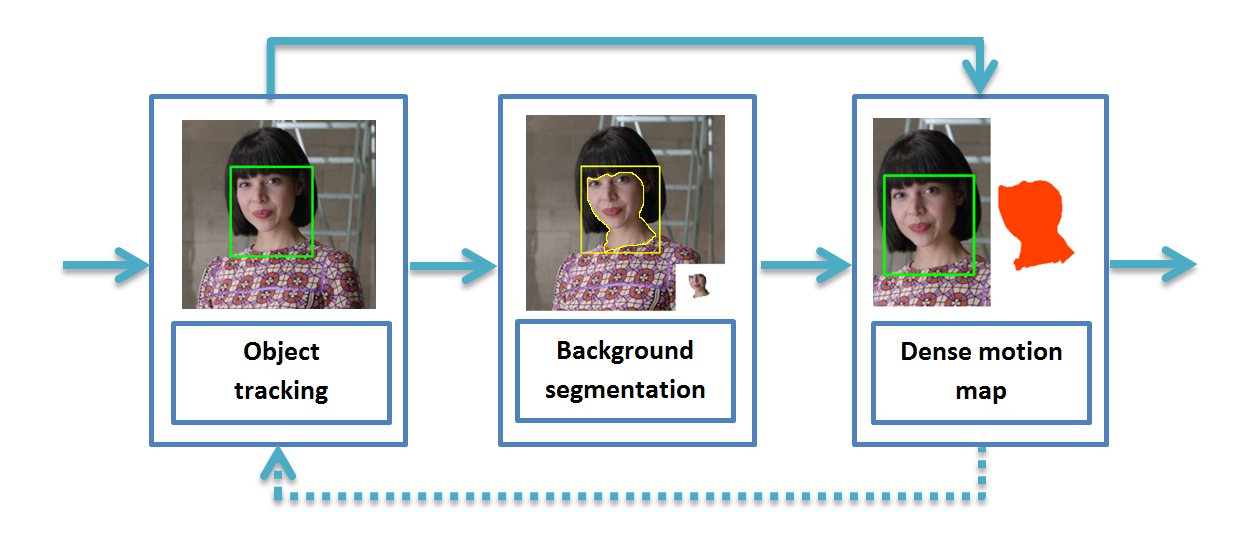
\includegraphics[width=1.00\textwidth]{../images/system.png}
      \caption{Block diagram of the proposed pipeline.}
      \label{figurelabel_sys}
   \end{figure}

The first step in the object flow pipeline can be selected according to specific need for a given application. We prefer, in general, tracking-by-detection methods 
like $Struck$ \cite{c22} or $MIL$ \cite{c23}, but other approaches could be followed. In the second place, for the object segmentation in video we propose the use 
of labelled background regions through the concept of superpixel flow, which is explained in the next section. Finally, the flow motion field is computed within the segmentation boundaries and long term dense 
point trajectories may be extracted from this.


\section{Conclusions}

A framework to combine tracking and optical flow methods to improve 
object based dense motion description is presented. The pipeline is 
composed of three main steps, object tracking, segmentation and 
flow estimation. For the segmentation step a new promising video object 
segmentation algorithm was proposed, and, to the best of our knowledge, 
the introduced superpixel flow is the first energy based algorithm for superpixel matching.
For the last step, we presented a flow estimation method based on a modification of the simple-flow method to use 
the obtained segmentation mask. The experiments showed that this object based flow estimation improves the dense motion 
estimation for an object in comparisson to optical flow techniques.
Future work includes to explore the use of the object flow as feedback hint for tracking-by-detection methods. 
Furthermore, the use of other optical flow techniques as base of the object flow is a matter of great interest as more precise methods could be found.
Finally, several kind of applications of the object flow can be more deeply approached. For instance, 
in the structure-from-motion pipeline, video editing and video inpainting, among others.



%A method for superpixel matching in a flow-like
%behavior had been presented. We may call it superpixel propagation, or super-pixel flow. This
%technique shows robustness in the labeling of the
%matches, and seems to be able to improve the results
%for object segmentation in video sequences when
%using the Grab-cut algorithm. Another motivation for
%this technique, however may be as initialization of
%optical flow techniques, to obtain more robust results
%due to a good initial guess for energy minimization
%methods. This has to be looked at more deeply in future work.
%===========================================================
\bibliographystyle{splncs}
\begin{thebibliography}{99}

\bibitem{c1}
J. Malik and X. Ren, Learning a classification model for segmentation, {\it Computer Vision, International Conference}, 2003.

\bibitem{c2}
S. Boltz; F. Nielsen and S. Soatto, Earth mover distance on superpixels, {\it International Conference on Image Processing}, 2010.

\bibitem{c3}
E. Boros; P. Hammer and G. Tavares, Preprocessing of unconstrained quadratic binary optimization, {\it RUTCOR}, 2010.

\bibitem{c4}
E. Boros and P. Hammer, Pseudo-boolean optimization, {\it Discrete applied Mathematics.}, 2002.

\bibitem{c5}
B. Horn and B. Schunck, Determining Optical Flow, {\it Artificial Intelligence}, 1981.

\bibitem{c6}
H. Ishikawa and P. Bouthemy, Multimodal estimation of discontinous optical flow using Markov random fields, {\it TPAMI.}, 1993.

\bibitem{c7}
V. Lempitsky, S. Roth and C. Rother, Fusion Flow: Discrete-Continuos optimization for optical flow estimation, {\it Computer Vision and Pattern Recognition}, 2008.

\bibitem{c8}
M. Reso and J. Jachalsky, Temporally Consistent Superpixels, {\it International Conference Computer Vision.}, 2011.

\bibitem{c9}
R. Achanta; A. Shaji; K. Smith; Aurelien Lucchi; P. Fua and S. Susstrunk, SLIC Superpixels compared to state of the art superpixel methods, {\it Discrete applied Mathematics.}, 2002.

\bibitem{c10}
F. Perbet and A. Maki, Homogeneus superpixels from random walks, {\it MVA.}, 2011.

\bibitem{c11}
C. Xu and J.J. Corso. Evaluation of super-voxel methods for early video proccesing, {\it Computer Vision and Pattern Recognition}. 2012.

\bibitem{c12}
A. Shekhovtsov, I. Kovtun and V. Hlavac. Efficient MRF deformation model for non-rigid image matching, {\it Computer Vision and Pattern Recognition}. 2007.

\bibitem{c13}
J. Sun, N.N Shen and H.Y. Shum. Stereo matching using propagation belief, {\it TPAMI}. 2003.

\bibitem{c14}
C. Rother, V. Kolmogorov and A. Blake. Grabcut: Interactive foreground extraction using iterated graph cuts, {\it SIGGRAPH}. 2004.

\bibitem{c15}
L. Yang, Y. Guo, X. Wu and X. Wang. A new video segmentation approach: Grabcut in local window,  {\it Soft Computing and Pattern Recognition}. 2011.

\bibitem{c16}
Y. Wu, J. Lim and M.-H. Yang. Online object tracking: A benchmark, {\it Computer Vision and Pattern Recognition}. 2013.

\bibitem{c17}
S. Baker, D. Scharstein, J.P. Lewis, S. Roth, M.J. Black and R. Szeliski. A Database and Evaluation Methodology for Optical Flow, {\it International Journal Computer Vision}. 2013.

\bibitem{c18}
Y. Boykov, M-P. Jolly. Interactive Graph Cuts for Optimal Boundary \& Region Segmentation of Objects in N-D images, {\it International Conference on Computer Vision}. 2013.

\bibitem{c19}
W. Li, D. Cosker and M. Brown. An anchor patch based optimization framework for reducing optical flow drift in long image sequences, {\it Asian Conference on Computer Vision}. 2012.

\bibitem{c20}
T. Crivelli, P.-H. Conze, P. Robert, M. Fradet and P. Perez. Multi-step flow fusion: towards accurate and dense correpondence in long video shots, {\it British Conference Machine Vision}. 2012.

\bibitem{c21}
M. Tao, J. Bai, P. Kohli, and S. Paris. SimpleFlow: A Non-iterative, Sublinear Optical Flow Algorithm, {\it Computer Graphics Forum, Eurographics}. 2012.

\bibitem{c22}
Brox, A. Bruhn, N. Papenberg, J. Weickert. High accuracy optical flow estimation based on a theory for warping. {\it European Conference in Computer Vision}. 2004.

\bibitem{c23}
S. Hare, A. Saffari, and P.H.S. Torr, Struck: Structured Output Tracking with Kernels.  {\it International Conference on Computer Vision}. 2011.

\bibitem{c24}
B. Babenko, M.H. Yang, and S. Belongie. Visual Tracking with Online Multiple Instance Learning. {\it Computer Vision and Pattern Recognition}. 2009.

\bibitem{c25}
J. Shi and C. Tomasi. Good features to track. {\it Conference on Computer Vision and Pattern Recognition }, 1994. 


\end{thebibliography}
%===========================================================

\end{document}
